\documentclass{article}

\usepackage{graphicx}
\usepackage{tikz}
\usepackage{tikzsymbols}
\usetikzlibrary{calc,patterns,shapes.geometric}
\pagestyle{empty}
\usepackage[margin=0pt]{geometry}
\geometry{papersize={14in,12in}}

\def\centerarc[#1](#2)(#3:#4:#5){\draw[#1] ($(#2)+({#5*cos(#3)},{#5*sin(#3)})$) arc (#3:#4:#5);}

\begin{document}
	\begin{figure}
		\centering
		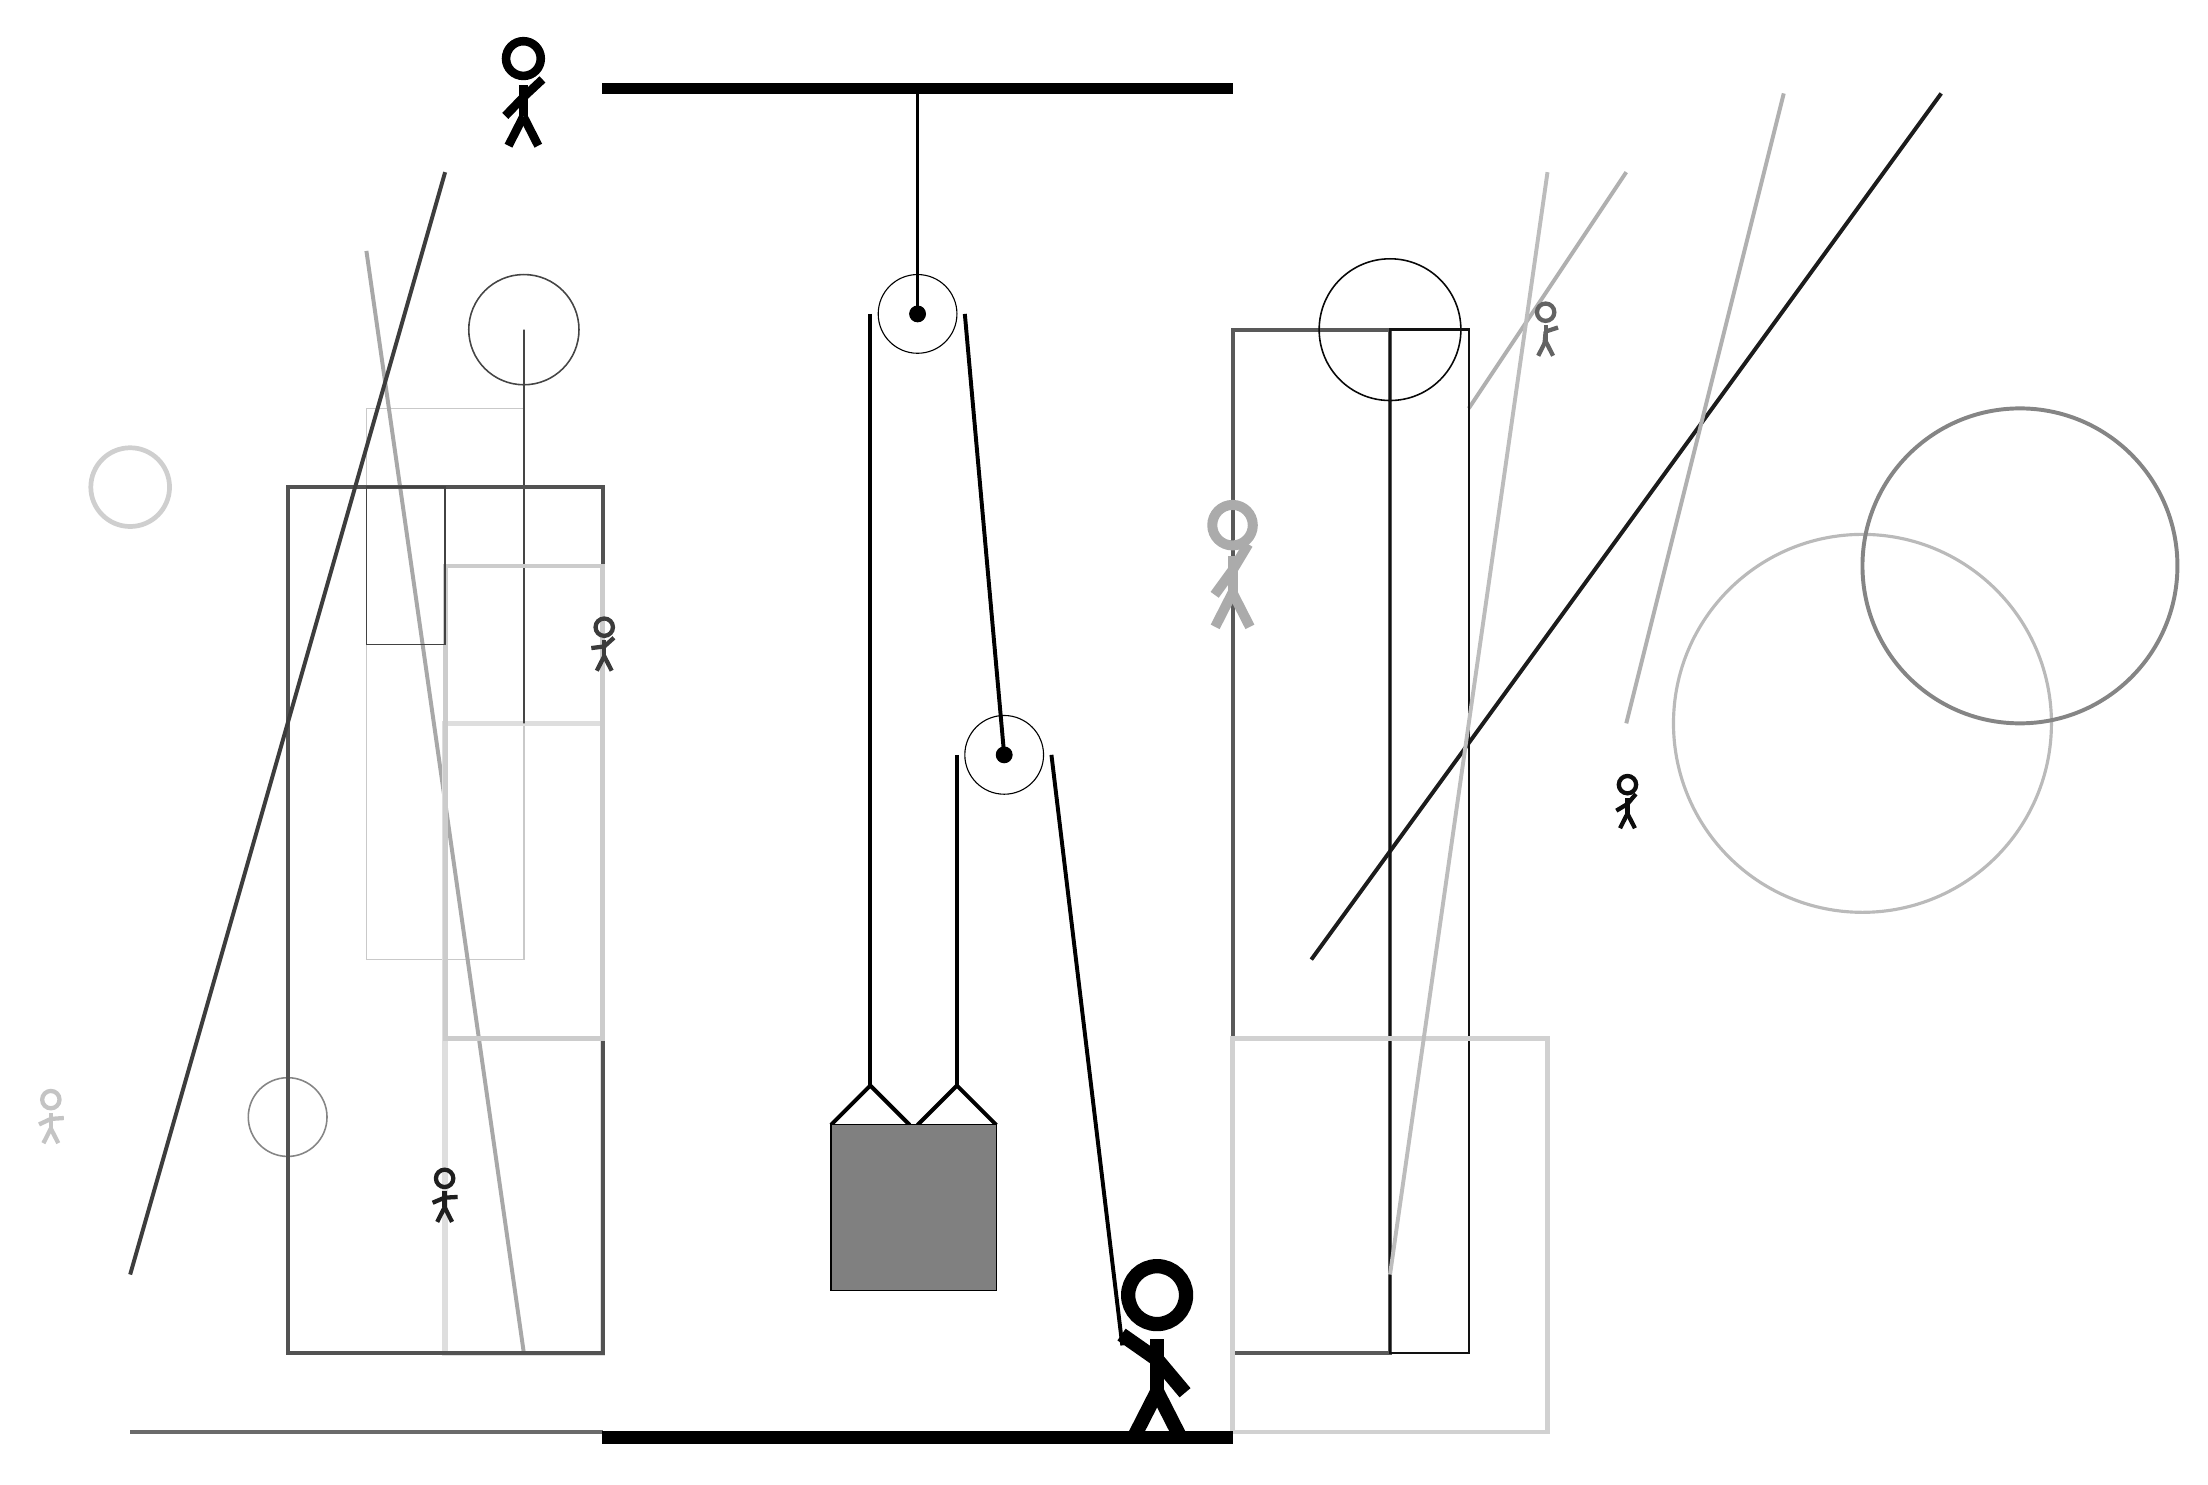
\begin{tikzpicture}
			%%%%% START %%%%%
			
			\draw[fill=black] (-2, 14) rectangle (6, 14.125);
			
			\draw (2, 11.2) circle (0.5);
			\draw[fill=black] (2, 11.2) circle (0.1);
			\draw[thick] (2, 11.2) -- (2, 14);
			
			\draw (3.1, 5.6) circle (0.5);
			\draw[fill=black] (3.1, 5.6) circle (0.1);
			
			\draw[line width = 0.5mm]  (0.9, 0.9) -- (1.4, 1.4) -- (1.9, 0.9);
			\draw[line width = 0.5mm]  (2.0, 0.9) -- (2.5, 1.4) -- (3.0, 0.9);
			\draw[fill=black!50] (0.9, 0.9) rectangle (3.0, -1.2);
			
			\draw[line width = 0.5mm] (1.4, 11.2) -- (1.4, 1.4);
			\centerarc[line width = 0.5mm](2, 11.2)(0:180:0.6);
			\draw[line width = 0.5mm] (2.6, 11.2) -- (3.1, 5.6);
			\draw[line width = 0.5mm] (2.5, 5.6) -- (2.5, 1.4);
			\centerarc[line width = 0.5mm](3.1, 5.6)(0:180:0.6);
			\draw[line width = 0.5mm] (3.7, 5.6) -- (4.6, -1.9);
			
			\draw[line width=0.5mm, color=black!65] (6, 11) rectangle (8, -2);
			
			\draw[line width=0.2mm, color=black!21] (-3, 3) rectangle (-5, 10);
			\draw [line width=0.2mm, color=black!48](-6, 1) circle (0.5);
			\draw[line width=0.5mm, color=black!89](7, 3) -- (15, 14);
			
			\draw[line width=0.5mm, color=black!31](11, 13) -- (9, 10);
			\draw[line width=0.5mm, color=black!34](-5, 12) -- (-3, -2);
			
			\draw[line width=0.7mm, color=black!13] (-2, -2) rectangle (-4, 6);
			\draw[line width=0.5mm, color=black!58](-2, -3) -- (-8, -3);
			\draw [line width=0.2mm, color=black!97](8, 11) circle (0.9);
			\draw [line width=0.6mm, color=black!19](-8, 9) circle (0.5);
			
			\draw[line width=0.2mm, color=black!73] (-3, 6) rectangle (-3, 11);
			\draw [line width=0.4mm, color=black!27](14, 6) circle (2.4);
			\node[line width=0.2mm, color=black!88] at (-4, 0) {\Strichmaxerl[3][23][3]};
			
			\draw[line width=0.5mm, color=black!68] (-2, 9) rectangle (-6, -2);
			\draw[line width=0.6mm, color=black!20] (-2, 2) rectangle (-4, 8);
			\draw [line width=0.5mm, color=black!48](16, 8) circle (2.0);
			
			\draw [line width=0.2mm, color=black!73](-3, 11) circle (0.7);
			\node[line width=0.3mm, color=black!61] at (10, 11) {\Strichmaxerl[3][85][18]};
			\draw[line width=0.5mm, color=black!76](-4, 13) -- (-8, -1);
			\draw[line width=0.3mm, color=black!93] (8, 11) rectangle (9, -2);
			\draw[line width=0.5mm, color=black!31](11, 6) -- (13, 14);
			
			\node[line width=0.6mm, color=black!100] at (-3, 14) {\Strichmaxerl[6][46][43]};
			\node[line width=0.4mm, color=black!95] at (11, 5) {\Strichmaxerl[3][31][50]};
			\node[line width=0.7mm, color=black!77] at (-2, 7) {\Strichmaxerl[3][7][42]};
			\draw[line width=0.2mm, color=black!74] (-4, 9) rectangle (-5, 7);
			
			\node[line width=0.7mm, color=black!33] at (6, 8) {\Strichmaxerl[7][54][59]};
			
			\node[line width=0.2mm, color=black!23] at (-9, 1) {\Strichmaxerl[3][25][4]};
			\draw[line width=0.6mm, color=black!18] (6, -3) rectangle (10, 2);
			
			\draw[line width=0.5mm, color=black!26](8, -1) -- (10, 13);
			
			\node at (5, -2) {\Strichmaxerl[10][-35][-50]};
			
			\draw[fill=black] (-2, -3) rectangle (6, -3.15);
			
			%%%%% END %%%%%
		\end{tikzpicture}
	\end{figure}	
\end{document}